%

% TODO: SDF vs SFD typo factory!

\documentclass[twocolumn]{amsart}
\usepackage[top=0.75in, left=0.65in, right=0.65in, bottom=0.6in]{geometry}

\usepackage{url}
% \usepackage{code}
% \usepackage{cite}
\usepackage{latexsym}
\usepackage{amsmath}
\usepackage{amssymb}
\usepackage{graphicx}
\usepackage{chessboard}
% IPA symbols. safe turns off overrides for like \! which I still want
\usepackage[safe]{tipa}

% \usepackage{chessfs}
\usepackage{adjustbox}

\usepackage[most]{tcolorbox}

\interfootnotelinepenalty=0

% lets me explicitly set a. or 1. etc. as enum label
\usepackage{enumitem}

\pagestyle{empty}

\usepackage{ulem}
% go back to italics for emphasis, though
\normalem

\usepackage{natbib}

\setlength{\footnotesep}{2em}

% \newcommand\comment[1]{}
\newcommand\sfrac[2]{\!{}\,^{#1}\!/{}\!_{#2}}

\begin{document}

\title{Lowestcase and Uppestcase letters: Further adventures in Derp Learning}
\author{Dr.~Tom~Murphy~VII~Ph.D.}\thanks{
Copyright \copyright\ 2021 the Regents of the Wikiplia Foundation.
Appears in SIGBOVIK~2021 with the
OS2TypoLinegap of the Association for Computational Heresy; {\em IEEEEEE!}
press, Verlag-Verlag volume no.~0x40-2A. 1 em}

\setchessboard{showmover=false}

\newcommand\makelowercase{{\sf make\_lowercase}}
\newcommand\makeuppercase{{\sf make\_uppercase}}

\renewcommand\th{\ensuremath{{}^{\textrm{th}}}}
\newcommand\st{\ensuremath{{}^{\textrm{st}}}}
\newcommand\rd{\ensuremath{{}^{\textrm{rd}}}}
\newcommand\nd{\ensuremath{{}^{\textrm{nd}}}}
\newcommand\at{\ensuremath{\scriptstyle @}}

\date{1 April 2021}

\maketitle \thispagestyle{empty}

\sloppypar


\section{Introduction}

Have you ever been writing something on the internet and wanted to convey
that you ARE FEELING ANGRY? Conversely, have you ever fired back a super
quick dm and u wanted to make it clear that it was like super ca\textipa{Z}
and so u didnt use ne capitals or punctuation dots except 4 that one place
where u needed to use the international phonetic alphabet because u dont
no how to write ca\textipa{Z} as in short for casual without it lol

If so, you made use of the fact that all letters have UPPERCASE
VERSIONS (e.g.~signifying ANGER) and lowercase versions
(e.g.~signifying u dont care lol). These dimensions have other uses,
for example, it is polite to start a person's name with a capital
letter to show that you took the time to regard their humanity (as it
takes extra work to press the caps lock key, press the first letter of
their name, and then press ther caps lock key again to turn it off).
In German, Nouns start with uppercase Letters, signifying Superiority
over other grammatical Categories like Verbs and Adjectives. Lowercase
letters can be used to conserve printer ink. Actually, I'm not sure that
lowercase letters have any other uses, but let's just roll with it.

The thing is: What if I'm even MORE ANGRY THAN I WAS BEFORE? There are
some standard sorts of typographic emphasis, like I can be {\bf BOLD
  ANGRY} or \textbf{\textit{\large BIG BOLD ITALIC UNDERLINE ANGRY}}
or { \Large \textbf{\textit{\uuline{COMBINE A LOT OF THESE ANGERS}}}},
each with its own nuances, depending on the cascading style sheet or
LaTeX class file. To be even more casual than lowercase, u can learn 2
write like this, and {\scriptsize shrink away} and also \sout{cross
  out ur words in shame in advance of them even being read}, but there
are few other options for de-emphasis. Plus, when I'm FEELING PRETTY
ANGRY, TOM, how do I capitalize that already-capitalized T in order to
show the proper reverence for your humanity?

This paper is about unshackling this dimension of human expression by
introducing letterforms further along the uppercase and lowercase
dimensions. Basically, we want to know what the upper{\it er}case
version of uppercase T is, and a lower{\it er}case version of
lowercase t is.

\subsection{Induction}

Today we're just concerned with English letters, of which there are
only 26. To create an upperercase and lowerercase alphabet by hand is
O(52 pick up), which for a guy who likes drawing letters anyway and
who alphabetized Star~Wars for fun, is not much to ask. In fact I
drew such alphabets in Figure~\ref{fig:manual} just now.

\begin{figure}[ht]
% \includegraphics[width=0.9 \linewidth]{manual}
\caption{TODO} \label{fig:manual}
\end{figure}

But, why do easy fun things by hand when you can build a complicated
automatic solution which produces much worse results? Well, there is
no good reason. I could claim that this allows us to automatically
upperercase any font, which is true, but the results are at best
moderately letter-like lumps. In principle there are several other
interesting things we can do, like apply the function over and over to
approach the uppestcase and lowestcase letters. This sounds fun, but
the results themselves are not going to impress. But the story of
getting there may be interesting, and even as it turns out to be
``derp learning,'' there will be opportunities for more good puns. So
let's just roll with it!


\section{Capital A Artificial Intelligence}

% XXX introduce the meaning of the \letterform syntax somewhere?

\newcommand\letterform[1]{\tcbox[
    nobeforeafter,
    tcbox raise base,
    top=0pt,bottom=0pt,left=-1pt,right=-1pt,
    left skip=1pt,
    right skip=1pt,
    arc=2pt,outer arc=2pt,
    boxrule=0.15mm,
    colback=white,
    colframe=white!50!black
    ]{\textrm{#1}}}

%     leftrule=0.2pt,rightrule=0.2pt,toprule=0.2pt,bottomrule=0.2pt,
%     enhanced jigsaw,
%    borderline horizontal={0.2pt}{0pt}{dashed},
%    borderline vertical={0.2pt}{0pt}{dashed}


We want to machine-learn two functions, \makelowercase\ and
\makeuppercase. Each takes a letterform and returns a letterform (we
can choose how these are represented) and does the needful, e.g.
\makelowercase(\letterform{A}) should return \letterform{a}. In order to learn this function, we'll at least need a lot of
examples to use as training data. A training example for
\makelowercase\ is a letterform and its expected corresponding
lowercase one. We can ``easily'' find a large amount of examples by
using existing fonts, and pairing their \letterform{A} with their
\letterform{a}, and so on for all 26 letters, and symmetrically for
\makeuppercase.

However, if we only give uppercase letters to \makelowercase, it
may very well learn how to generate the corresponding lowercase letter
but be unable to do anything interesting for other letterforms. This
is a problem because we want to use this function to see
what e.g.~\makelowercase(\letterform{a}) is.

This is not (only) the problem of overfitting. An overfit model could
work well on the letter \letterform{A} from one font (because it has
seen that font before) but fail on \letterform{A} from a new font. The
property that we want is that the learned function can also produce an
interesting result on a shape it's never seen before, like
\letterform{\textipa{Z}}\,. That is, it has generalized the idea of
``how to make a shape lowercase,'' not simply ``how to make a capital
A shape lowercase.''

The problem with this is that we don't have any training data other
than existing fonts to tell us what the lowercase of some arbitrary
shape should look like. Without examples of this form, the problem is
unconstrained. \makelowercase\ could learn to generate empty output
for anything it doesn't recognize as a capital letter, and still have
perfect performance on the training and test set. It is hard to
generate training data of this form (even by hand) as we don't have
much idea {\em a priori} of what a lowerercase \letterform{a} should
look like (except for e.g.~One Artist's Impression from
Figure~\ref{fig:manual}).

\newcommand\trainingexample[2]{$\langle$\letterform{#1}$,\,$\letterform{#2}$\rangle$}

\newcommand\weirdcharlo{
\includegraphics[width=0.75em]{weirdchar-lo}}
\newcommand\weirdcharup{
\includegraphics[width=0.75em]{weirdchar-up}}
\newcommand\lowerlowera{
\includegraphics[width=0.6em]{lowerlowera}}

This brings us to the one decent idea in this paper (which by the way
only sort of works, but let's just roll with it). We can at least
express one characteristic property of the \makelowercase\ function
that ought to be true even for letterforms we don't have examples of:
It ought to be the inverse of \makeuppercase. So, we train these two
models in tandem. \makelowercase\ is fed training examples from the
sample fonts like \trainingexample{Q}{q} etc.~and \makeuppercase\ gets
\trainingexample{e}{E} etc.~as expected. We also run the current
version of \makeuppercase\ on some letter-like shapes, which produces
some other shape. For example, say that
\makeuppercase(\letterform{\weirdcharlo}) outputs
\letterform{\weirdcharup}. We have no idea if this is good or not, so
we don't update the model. However, we {\em do} provide the training
example to \trainingexample{\weirdcharup}{\weirdcharlo} to the
\makelowercase\ training queue and penalize {\em it} if it did not
predict \letterform{\weirdcharup}. In this way, whatever \makeuppercase\ is
doing, we ask \makelowercase\ to learn the inverse. We of course also
simultaneously do the symmetric thing, using the output of
\makelowercase\ to create training examples for
\makeuppercase\ (Figure~\ref{fig:cotraining}).



\begin{figure}[ht]
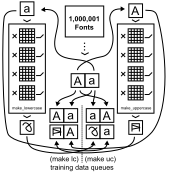
\includegraphics[width=0.9 \linewidth]{training}
\caption{ Simultaneously training the two models. This example
  illustrates how a pair of letterforms \letterform{A} and
  \letterform{a} from the same font becomes four training examples.
  The pair straightforwardly generates an example
  \trainingexample{A}{a} for the \makelowercase\ queue, and an example
  \trainingexample{a}{A} for the \makeuppercase\ queue. Separately, we
  supply \letterform{a} to the \makelowercase\ model, simply to get
  the current output \letterform{\lowerlowera} (no model updates are
  performed). But this pair reversed becomes a training example
  \trainingexample{\lowerlowera}{a} for the \makeuppercase\ queue.
} \label{fig:cotraining}
\end{figure}

Because \makelowercase\ is getting training examples of
uppercase/lowercase pairs from real fonts, it remains grounded on real
letters. It is also free to generate new shapes for the open domain
(outside \letterform{A}--\letterform{Z}). However, it is penalized if
its behavior is not the inverse of whatever \makeuppercase\ is
currently doing. And since we do the symmetric thing for
\makeuppercase\, there is a (slow) feedback loop between the two
models that keeps them from straying too far from the grounded
examples. The idea is that this allows them to do some creative
generalization outside their native domains, but in a way that
still has some constraint.

In practice, we don't feed arbitrary shapes to the models. We just
need something letter-like, and in fact we have a large collection of
letter-like shapes among our existing fonts! We pass already-lowercase
shapes to \makelowercase, in order to generate inversion examples for
training \makeuppercase. These shapes are clearly letter-like (they
{\em are} letters) and are also of interest to us anyway, since we
want to try to generate lowerercase and upperercase letters from
the trained models.


\section{1000001 Free Fonts}

Sprechen of fonts, I downloaded every font I could find on the whole
internet. This was overkill. The resulting directory tree contained
over 100,000 files, many of which were duplicates. Exact duplicates
are easy to find, but since many of these files were the result of 30
years of community transmission, they had acquired various mutations.
One of the first things I did was write software to automatically
remove files that were essentially duplicates even if they weren't
exactly the same bytes.

Next, my lord, do people have bad taste! And I say this as someone who
made dozens of amateurish fonts\cite{dbzfonts} as a high school and
college student and who is contributing several new questionable
fonts\label{sec:newfonts} as a result of this paper. The database is
just filled with garbage that is unusable for this project: Fonts that
are completely illegible, fonts that are missing most of their
characters, fonts with millions of control points, Comic Sans MS,
fonts where every glyph is a drawing of a train, fonts where
everything is fine except that just the lowercase r has a width of
{\tt MAX\_INT}, and so on. So I built a UI
(Figure~\ref{fig:sortition}) for efficiently and mind-numbingly
cleaning up the database by marking fonts as broken or suitable (and
also categorizing them as serif, sans-serif, decorative, techno, etc.,
which I never used). In doing this I noticed another extremely common
problem, which was that many fonts had the same letter shapes for
uppercase and lowercase letters. This would not do for the current
application!

\begin{figure*}[ht]
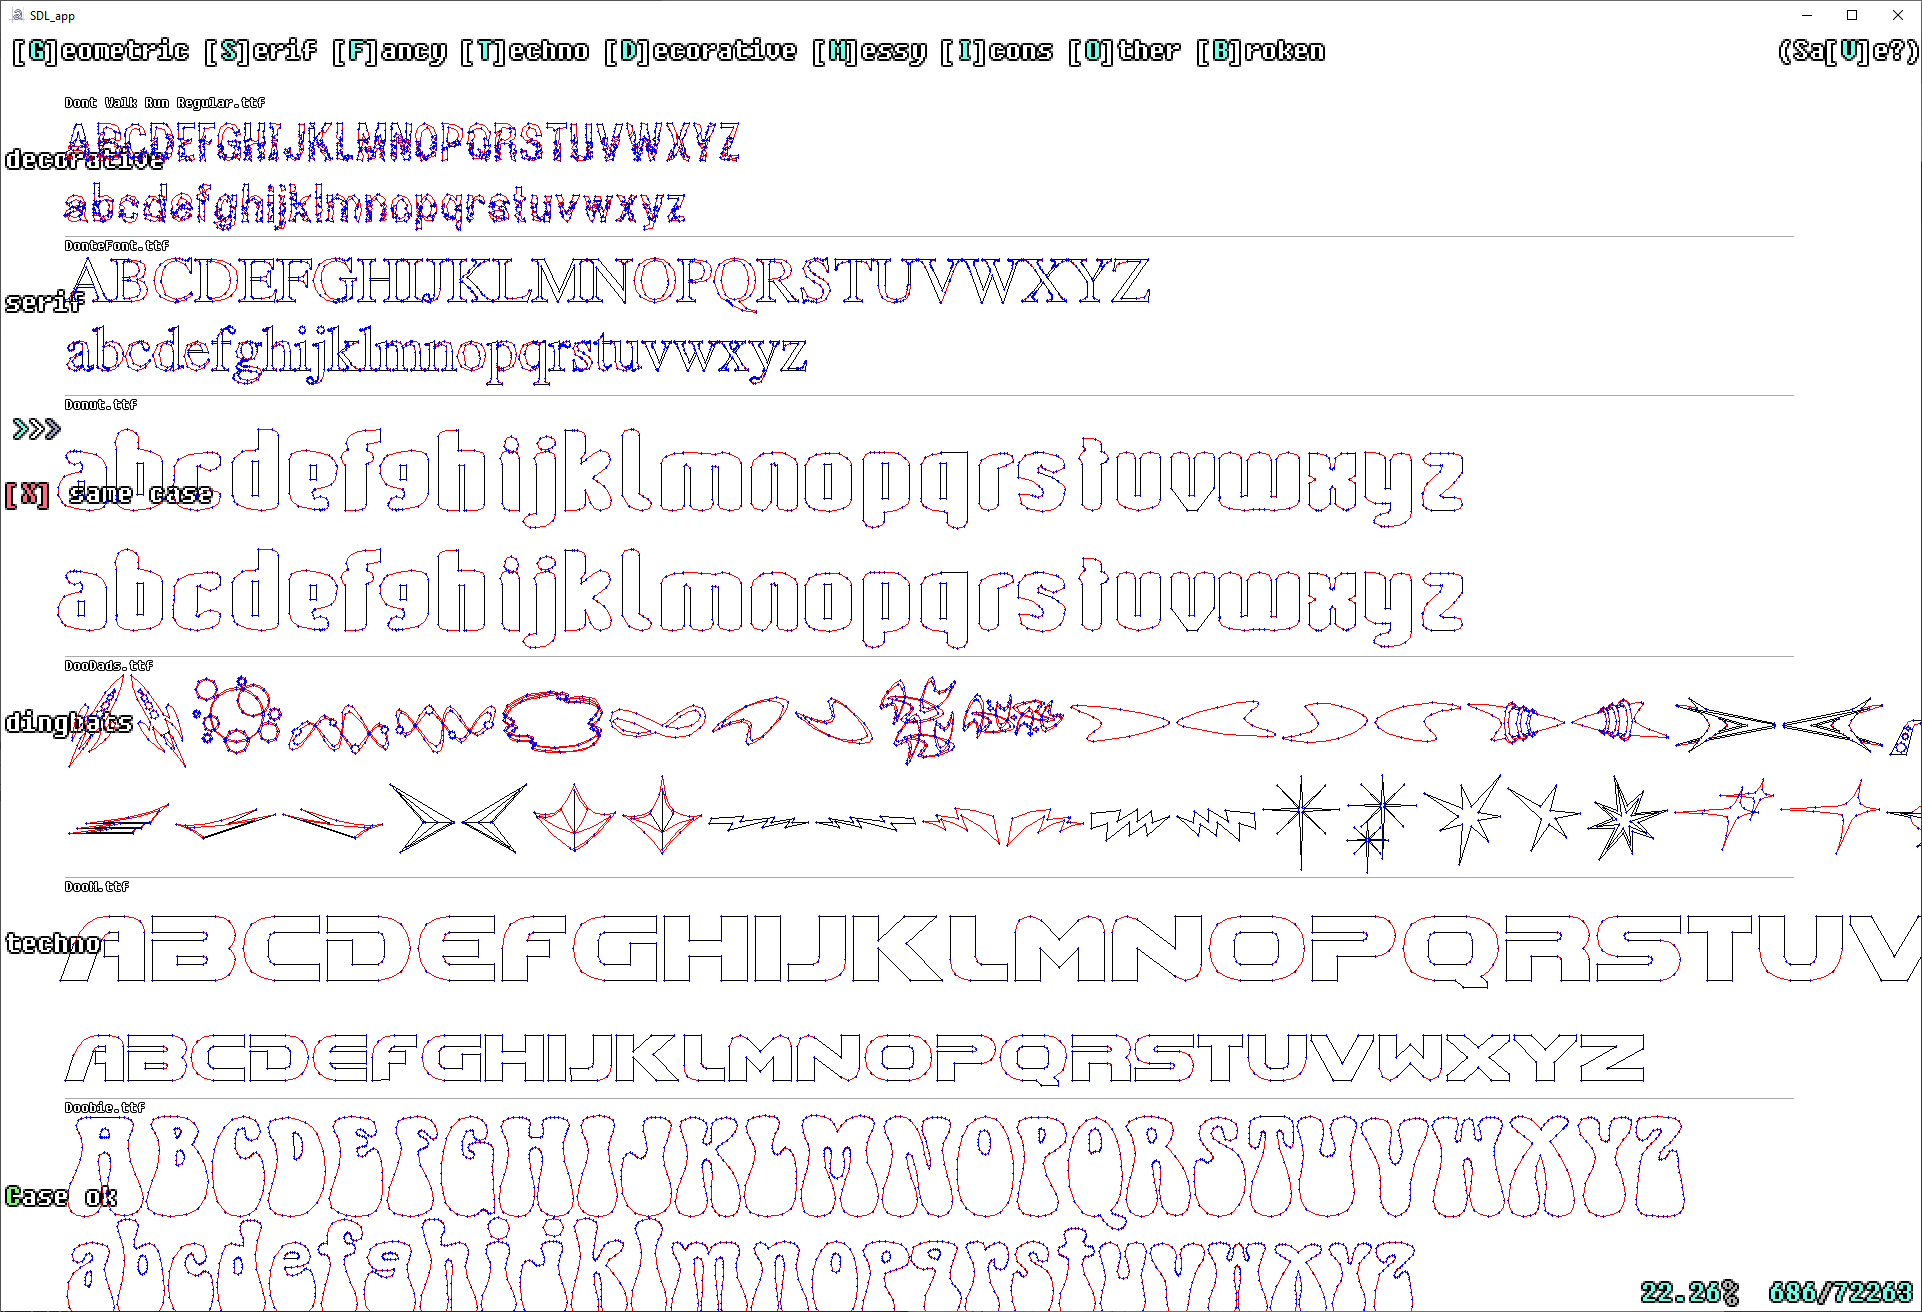
\includegraphics[width=0.9 \linewidth]{sortition}
\caption{ The interactive font data-cleaning UI. A seemingly endless
  series of fonts presents, with single keypresses putting the fonts
  into common categories such as (b)roken.
  % XXX maybe write more?
} \label{fig:sortition}
\end{figure*}

But why manually mark fonts with nearly the same upper- and
lowercase letters, when you could build a complicated automatic
solution? The first pass identified fonts whose letters were
exactly the same, but this was only a small fraction of the
problematic fonts. A common issue was that the lowercase characters
were very slightly modified versions of the uppercase ones, often
scaled and translated and then perhaps ``optimized'' during the
font export.

So, for a given font, I want to reject it if for most pairs of cased
letters \letterform{A},\letterform{a}, \letterform{a} is close to a
linear transformation of \letterform{A}. This problem can probably be
solved with math, but it didn't sound that fun. Instead I tried out
a new tool, and it worked well enough that I've now added it to the
permanent rotation: Black-box function optimizers.

\paragraph{Black-box optimization.} If you have a function and want
to find arguments that minimize its output, the most efficient
techniques are generally those like gradient descent. (In fact, the
backpropagation algorithm we use to training the neural network in
Section~\ref{sec:neural} is gradient descent on the function that
takes the model weights and produces an error value for each output
node.) The problem with this is that you need to do some math to
compute the gradient function, and anyway you need to deal with fiddly
bits (Section~\ref{sec:fiddly}) unless the function is convex and
smooth, which it will not be. If you don't want to deal with that,
and have a fast computer (and who doesn't?), black-box optimization
algorithms are worth considering. Here, the interface\footnote{
  Here a simplfied wrapper around BiteOpt~\cite{biteopt} in my {\tt cc-lib}
  library. See \url{https://sourceforge.net/p/tom7misc/svn/HEAD/tree/trunk/cc-lib/opt/}.}
  is just something like (C++):

\begin{verbatim}
  double Minimize1D(
      const std::function<double(double)> &f,
      double lower_bound,
      double upper_bound,
      int iters);
\end{verbatim}

which takes a function \verb+f+ of type \verb+double+ $\rightarrow$
\verb+double+, finite bounds on the argument's value, the maximum
number of times to call that function, and returns the argument it
found that produced the minimal value. Not as fast as gradient
descent, but in practice ``if the function is kinda smooth'' these
optimizers produce excellent results! The chief selling point for me
is that I don't need to think about anything except for writing the
function that I want minimized, which I just express in normal code.

\begin{figure}[ht]
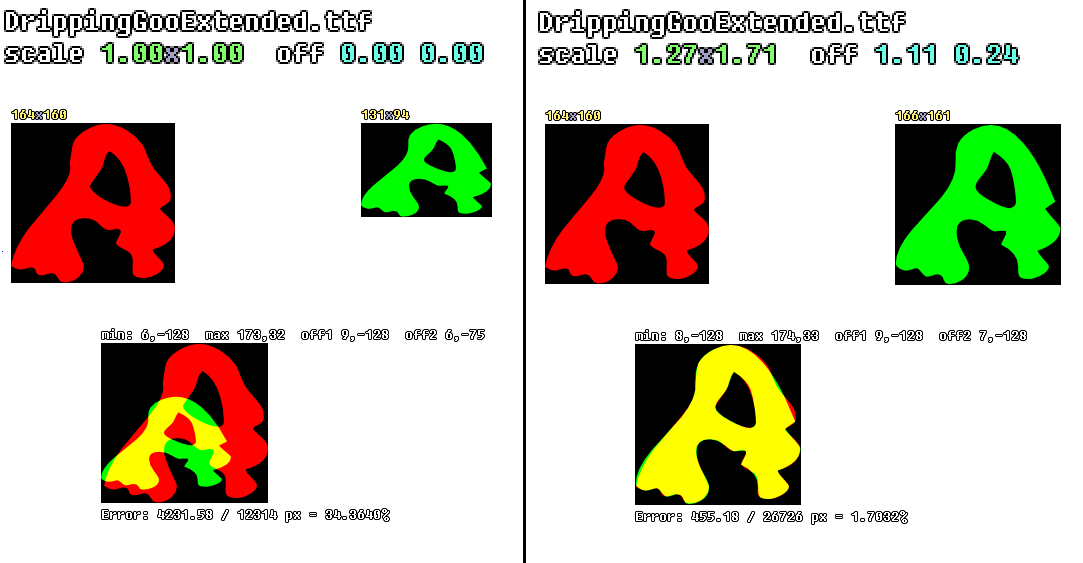
\includegraphics[width=0.9 \linewidth]{casealignment}
\caption{ Example alignment to reject the font
  {\tt DrippingGooExtended}.
  At left, \letterform{A} (red) and
  \letterform{a} (green) rendered with the identity transform, and
  their alignment ($35\%$ difference) below. At right, the transform
  found by the black-box optimizer and the resulting alignment with
  $1.7\%$ difference. Note that the shapes are still not an exact
  match (the export process has to round the data to integers and
  might apply other non-linear transformations like curve
  simplification), but these are clearly not a useful pair for
  the current problem.} \label{fig:casealignment}
\end{figure}

In this case, I render the letterform \letterform{A} and then optimize
a four argument function taking {\tt xoff}, {\tt yoff}, {\tt xscale},
{\tt yscale}. This function renders \letterform{a} with those
parameters, then just computes the difference in the two rendered
bitmaps. This finds the best alignment of the two letterforms (under
the linear transformation) in a few hundred milliseconds
(Figure~\ref{fig:casealignment}). If the disagreement is low as a
function of the total pixels, then we say that the letters have the
same case. If enough of them have the same case, we reject the font. I
set the thresholds by looking at the P/R curve computed on random
hand-labeled examples (Figure~\ref{fig:samecasepr}).

\begin{figure}[ht]
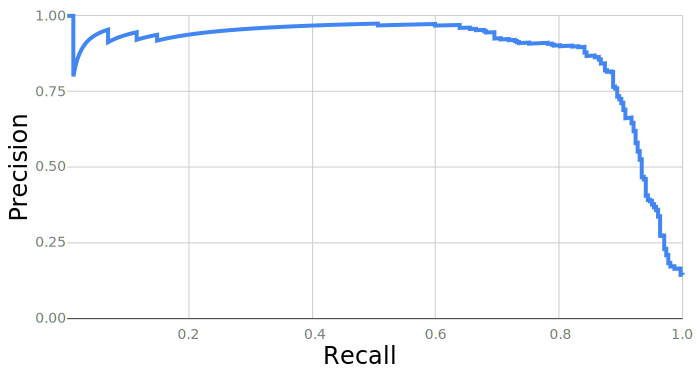
\includegraphics[width=0.9 \linewidth]{samecasepr}
\caption{ Precision--recall curve for automatically detecting fonts
  that have basically the same upper- and lowercase shapes. It's good!
  This is how you want 'em to look!
} \label{fig:samecasepr}
\end{figure}

\medskip

I labeled fonts using the UI until I had 10,000 that were clean enough
for a training set and passed the same-case heuristic.

\section{The simplest thing that might work} \label{sec:vectorversion}

Before getting fancy (which we we will) it's good engineering hygiene
to try the simpliest thing that might just work (it doesn't). Fonts
are represented as vector data (lines and quadratic B\'ezier curves).
Can we just train a network that takes these lines and curves as input
and predicts the lower- or uppercased letter in the same format? (No.)

We'll at least put the data in a somewhat normalized form. The neural
network will take a fixed number of inputs to a fixed number of
outputs, so a simple approach is to decide on some maximum number
control points per letter, and only try training on fonts whose
letterforms fit within that budget. Letterforms can be made of
multiple contours (e.g. a stacked \letterform{g} typically has two
holes in it, and \letterform{j} has two disjoint parts). I found that
most clean fonts had three or fewer contours, and when sorting them by
descending length, most fit within 38, 14, and 10 endpoints for the
three. So, I only train on fonts where all of the letters fit within
this budget.\footnote{It would not be a good idea to reject only the letters
that don't fit, because it might result in the network being trained
on more \letterform{l}s (tends to be simple) than \letterform{g}s
(tends to be complex).}

% TODO: Illustrate a letterform and its contours?

Rather than try to work with both lines and B\'ezier curves, I
normalize each contour to only contain B\'eziers, by turning a line
segment into an equivalent B\'ezier with its control point at the
midpoint. This frees us from having to distinguish the two types in
the data. We also need each of the three contours to not be {\em too
  short}, so I fill out the fixed-size buffers by repeating the last
point. This is not great but does have the correct meaning (bunch of
useless zero-length edges). It has the property that any predicted
data can be rendered and has a straightforward point-by-point error
function (which might not be the case if we were predicting a dynamic
number of points). Finally, I output the contour's points starting
from the point closest to the origin in order to reduce one needless
degree of freedom.

The network I trained has an input layer size of $154 = (38 + 14 + 10)
\times 4 + 3 \times 2$ (one control point and one end point per
B\'ezier curve), plus a starting point for each of the three contours.
The output layer is the same size, plus 26 (see below). There are
three hidden layers of size 308, 308, 360. The first layer is dense
and the remainder are sparse (two thirds to a half of the weights are
zero), for just about 1 million total parameters. All layers are leaky
rectified linear units. If you're taking notes, don't, as again this
does not work well, and I don't know how people figure out what the
right network size is anyway. I just made it up. You can give {\em me}
your notes.

\paragraph{Bonus outputs}. The output includes the predicted shape,
and also 26 individual predictors for each of the 26 letters. So a
training example is actually like \letterform{C} $\rightarrow$
\letterform{c} $[0, 0, 1, 0, 0, \ldots, 0]$, with the 1 in the third
place because C is the third letter. We don't need these outputs for
the problem itself (e.g. to lowercase new letter shapes), but there
are several ideas behind this. First, the lowercasing function we're
trying to learn does take into account the letter of the alphabet
being lowercased. By asking the network to learn this as well (it is
penalized when it gets the prediction wrong), it must learn features
that allow it to distinguish different letters, and those features are
available for use by outputs we {\em do} care about. This is an easy
way to coax it to learn features that I know are meaningful without
having to actually engineer feature extractors by hand (or first train
separate models, etc.). Perhaps the most useful thing is that it's
very clear what the right answer is, so it gives me an easy way to see
if the network is learning anything {\em at all}. (It does.) Finally,
we can do some silly stuff with these; see
Section~\ref{sec:hallucination}.

\newcommand\nan{\textsf{NaN}}
\renewcommand\inf{\textsf{inf}}

I trained the network using a home-grown (why??) GPU-based package
that I wrote for {\em Red i removal with artificial retina
  networks}~\cite{murphy2015redi}---an example of ``lowercase i
artificial intelligence''---and have improved as I repurposed it for
other projects, such as {\em Color- and piece-blind
  chess}~\cite{murphy2019blind}. It is ``tried and true'' in the
sense that ``every time I tried using it, I truly wanted to throw
my computer out the window, and retire to a hermitage in the glade
whenceforth I shall nevermore be haunted by a model which has
overnight become a sea of \inf{}s and \nan{}s.''

\begin{figure}[ht]
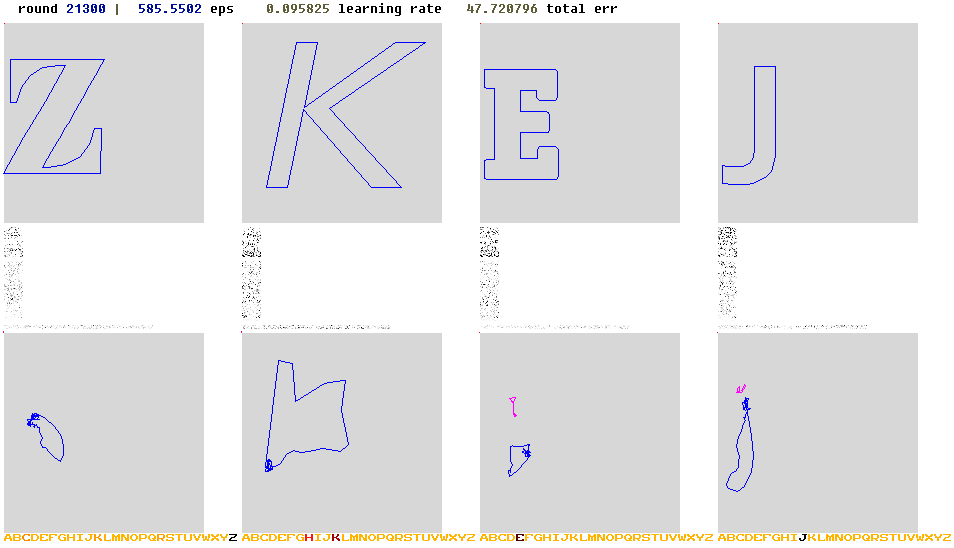
\includegraphics[width=0.9 \linewidth]{trainingvector}
\caption{ Screenshot of {\tt train.exe} running on the vector-based
  version of the problem. Shown is the \makelowercase\ model's output
  (bottom) on four shapes from four fonts (top). Some dust in between
  is the activation of the network's layers. At the very bottom, the
  26 predictions for ``what letter is this?''. The output for
  \letterform{j} is not too bad; you can see the distinct dot (a
  separate contour) and it sort of looks like a \letterform{j}. The
  \letterform{e} also has two pieces as expected but is otherwise
  garbage. The model is unsure whether the second input is an H
  or a K, and has predicted a shape sort of ambiguously between those
  two. The \lowercase{z} is also an embarrassment.
} \label{fig:trainingvector}
\end{figure}

I was so {\tiny confident} that this wouldn't work that I only trained
a \makelowercase\ model and didn't even worry about the more
complicated simultaneous training setup yet. I ran this for about
22,000 rounds, some 90 million training examples. Indeed it does not
work (Figure~\ref{fig:trainingvector}). It is not a total catastrophe,
though. The model can clearly recognize letters (though perhaps just by
memorization) and some of the shapes it generates are along the right
lines. ({\em Along the right lines}, get it??)

It's a bit hard on the

% TODO: Font file generated from this.
% TODO: Fitting the prediction to the actual in order to coax
% better results, failing.


% XXX cite futura
% XXX add downloadable font too
\begin{figure*}[tp]
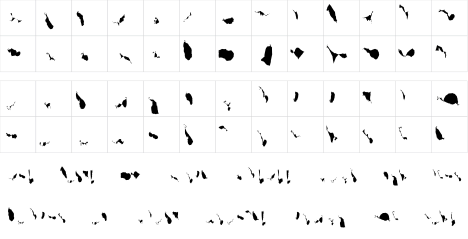
\includegraphics[width=0.9 \linewidth]{futurda}
\caption{ Type specimen for the generated font {\bf Futurda}. This is the
  classic font Futura, run through the vector based lowercasing model
  (Section~\ref{sec:vectorversion}). At top are Futura's letterforms
  \letterform{A}--\letterform{Z} run through the model and so ``made
  lowercase'' (it's obviously garbage). Next are the \letterform{a}--\letterform{z},
  made even more lowercase. Also rubbish.
  At the bottom are the pangrams ``Dr.~Jock, TV Quiz Ph.D., bags few lynx''
  and ``Sphinx of black quartz, judge my vow!'' Although the text is
  illegible and kind of uninteresting, it does have a certain dynamic
  Rorschach aesthetic, like a collection of delicate moths pinned
  to paperboard, that one could consider framing or publishing in
  the proceedings of SIGBOVIK 2021.
} \label{fig:futurda}
\end{figure*}


% lowerercase Franklin Gothic. Franklin mint... not guaranteed
% to go up in value


% the sdf problem

\section{The care and feeding of sparse matrices} \label{sec:neural}

\label{sec:fiddly}

% no copyright intended

% stretch the loss function near the onedge value

%

\section{Perfect letters, hallucinated}
\label{sec:hallucination}

% autotracing

% CAPS LOCK, LOCK, CAPTAIN'S LOCK

% when two letters coincide, a shift-reduce conflict

% cool s

% lowercase uppercase letters etc.

\nocite{murphy2019blind}
\nocite{murphy2019eloworld}

\bibliography{lowercase}{}
\bibliographystyle{plain}

\end{document}

